\documentclass[addpoints,spanish, 12pt,a4paper,cancelspace]{./include/gexam}

%%%%%%%%%%%%%%%%%%%%%%%%%%%
\renewcommand{\documentName} { Recuperación final junio }
\renewcommand{\documentContent} { 3º Evaluación } 
\renewcommand{\waterMark} { \phantom{Modelo A} } 

% Configuración del documento.
\renewcommand{\schoolSubject} { Examen Matemáticas 2º ESO  }
\renewcommand{\school} { IES José de Churriguera  }
\renewcommand{\academicPeriod} { Curso 2022/2023 }

\renewcommand{\autor} { Andrés Giménez Muñoz }
\renewcommand{\emailAuthor} { andresprofemates@outlook.es }
\renewcommand{\autorSing}{ Profesor: Andrés } 
%%%%%%%%%%%%%%%%%%%%%%%%%%%

%%%%%%%%%%%%%%%%%%%%%%%%%%%
% Exam configuration
%\pointsdroppedatright   %% No mostrar la puntuación
\pointsinrightmargin % Para poner las puntuaciones a la derecha. Se puede cambiar. Si se comenta, sale a la izquierda.
\extrawidth{-1.5cm} %Un poquito más de margen por si ponemos textos largos.
\marginpointname{ \emph{\points}}

%% Si se comenta no aparecerán los espacios de la solución.
%\nocancelspace

%% Esto es de la clase exam. Si dejamos sin comentar \printanswers, se mostraran las soluciones. 
%% Si la comentamos y dejamos sin comentar \noprintanswers, pues no se muestran las soluciones.
%\printanswers
%\noprintanswers

%%%%%%%%%%%%%%%%%%%%%%%%%%%

\begin{document}

\StudentData
\GradeTableHeader

\justifying

\begin{center}
    \fbox{\fbox{\parbox{6.5in}{             
                \begin{itemize}
                    \item Copiar, hablar, levantarse de la silla o molestar a al resto de la clase pueden ser motivos de la retirada del examen que se valorará con un cero.
                    \item Deben aparecer todas las operaciones, no vale solo con indicar el resultado.
                    \item Se podrán quitar hasta cinco décimas por falta de claridad o rigor en el desarrollo de las respuestas o por una mala presentación.
                    % \item Se valorará que se indiquen las cuentas en línea, realizando las operaciones en el margen.
                    \item Está permitido utilizar la calculadora.
                \end{itemize}
            }}}
\end{center}

\begin{questions}
    \setcounter{question}{0}

    \question[3] Obtén la ecuación de la recta que pasa por los puntos A(5,4) y B(6,2) 
    expresándola en su forma general y explicita.
    \vspace{\stretch{1}}

    \newpage

    \question[3] Dada la parábola $y = x^2 - 3x + 2$ calcula su vértice, punto de corte con los ejes de coordenadas 
    e indica si el vértice es un máximo o un mínimo.
    \vspace{\stretch{1}}
    
    \begin{center}
        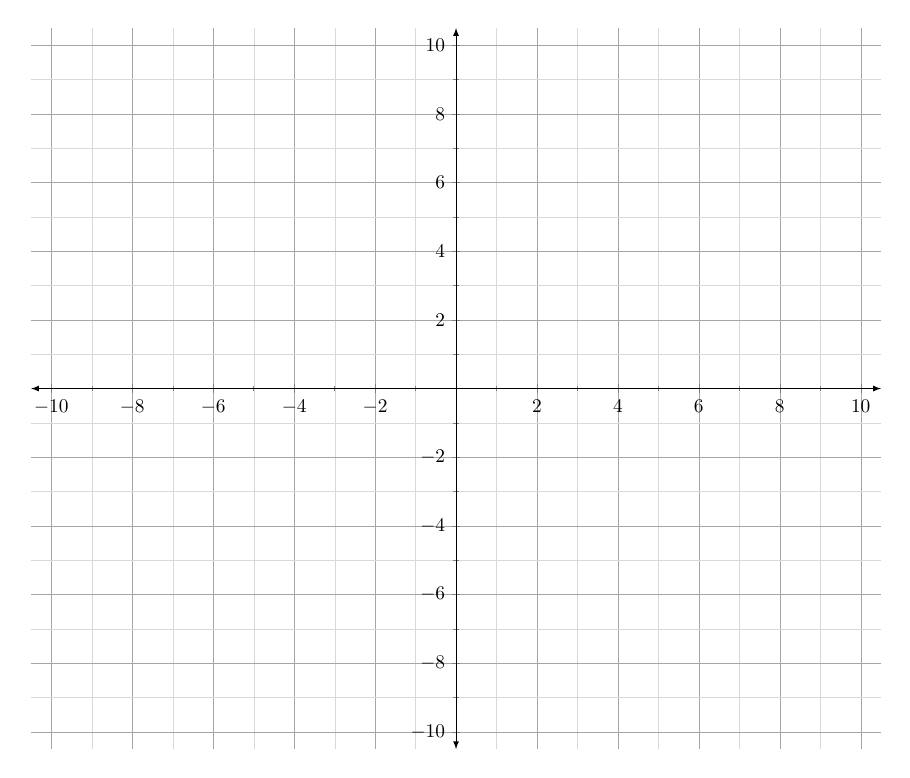
\begin{tikzpicture}[scale=0.7]
            \begin{axis}[
                axis x line=center,
                axis y line=center,
                xmin=-10,xmax=10,
                ymin=-10,ymax=10,
                grid=both,
                grid style={line width=.1pt, draw=gray!30},
                major grid style={line width=.2pt,draw=gray!70},
                axis lines=middle,
                axis line style={<->},
                minor tick num=1,
                enlargelimits={abs=0.5},
                axis line style={latex-latex},
                % ticklabel style={font=\tiny,fill=white},
                % xlabel style={at={(ticklabel* cs:1)},anchor=north west},
                % ylabel style={at={(ticklabel* cs:1)},anchor=south west},
                xlabel style={below right},
                ylabel style={above left},
                width=17cm,
            ]
        \end{axis}
        \end{tikzpicture}
    \end{center}

    \newpage
    \question[3] En un momento determinado del día la sombra de Juan mide $2,50m$ y la de un arbol $35m$, 
    sabiendo que Juan mide $1,75m$ ¿cuál es la altura del arbol?
    \\ \\
    \begin{minipage}{\linewidth}
        % \centering
        \includegraphics[width=7cm]{img01}
    \end{minipage}
    \vspace{\stretch{1}}

    \newpage 
    \question[1] Al dar una vuelta completa a la rueda de una bicicleta, está avanza $2,83m$ ¿Cuánto milímetros mide el diámetro de la rueda?
    \\ \\
    \begin{minipage}{\linewidth}
        % \centering
        \includegraphics[width=7cm]{img02}
    \end{minipage}
    \vspace{\stretch{1}}

\end{questions}
\end{document}